\documentclass{article}
\usepackage[utf8]{inputenc}
\usepackage[english, russian]{babel}

\usepackage{mathtext}
\usepackage[T2A, TS1]{fontenc}
\usepackage{microtype} % Slightly tweak font spacing for aesthetics
\usepackage{amsthm, amssymb, amsmath, amsfonts, nccmath}
\usepackage{nicefrac}
\usepackage{epstopdf}
\usepackage[export]{adjustbox}
\usepackage{float} % Improved interface for floating objects
\usepackage{graphicx, multicol} % Enhanced support for graphics
\usepackage{pdfrender,xcolor}
\usepackage{breqn}
\usepackage{mathtools}
\usepackage{titling}
\usepackage{bm}
\usepackage{centernot}
\usepackage[cal=boondoxo,calscaled=.96]{mathalpha}
\usepackage{marvosym, wasysym} % More symbols
\usepackage{rotating} % Rotation tools
\usepackage{censor} % Facilities for controlling restricted text
\usepackage{fancyhdr}

\usepackage{geometry} 
\geometry{left=2cm}
\geometry{right=1.5cm}
\geometry{top=1cm}
\geometry{bottom=2cm}

\begin{document}

\input titlepage

\tableofcontents
\addtocontents{toc}{~\hfill\textbf{Страница}\par}
\newpage
\listoffigures
\addtocontents{lof}{~\hfill\textbf{Страница}\par}
\newpage

\section{Постановка задачи}
Для 5 распределений:
\begin{itemize}
    \item Нормальное распределение $N(x, 0, 1)$
    \item Распределение Коши $C(x, 0, 1)$
    \item Распределение Лапласа $L(x, 0, \frac{1}{\sqrt{2}})$
    \item Распределение Пуассона $P(k, 10)$
    \item Равномерное распределение $U(x,-\sqrt{3},\sqrt{3})$
\end{itemize}
Сгенерировать выборки размером 10, 50 и 1000 элементов. Построить на одном рисунке гистограмму и график плотности распределения.

\section{Теория}
\subsection{Рассматриваемые распределения}
Плотности:
\begin{itemize}
    \item Нормальное распределение
    \begin{equation}\label{norm}
        N(x,0,1)=\frac{1}{\sqrt{2\pi}}e^{-\frac{x^2}{2}}
    \end{equation}
    \item Распределение Коши
    \begin{equation}\label{cauchy}
        C(x, 0, 1)=\frac{1}{\pi}\frac{1}{x^2+1}
    \end{equation}
    \item Распределение Лапласа
    \begin{equation}\label{laplace}
        L(x,0,\frac{1}{\sqrt{2}})=\frac{1}{\sqrt{2}}e^{-\sqrt{2}|x|}
    \end{equation}
    \item Распределение Пуассона
    \begin{equation}\label{poisson}
        P(k, 10)=\frac{10^k}{k!}e^{-10}
    \end{equation}
    \item Равномерное распределение
    \begin{equation}\label{uniform}
        U(x,-\sqrt{3},\sqrt{3})=
        \begin{cases}
        \displaystyle\frac{1}{2\sqrt{3}}&\text{при}\;\;|x|\:\leq\sqrt{3}\\
        \;\;\;0&\text{при}\;\;|x|\:>\sqrt{3}\\
        \end{cases}
    \end{equation}
\end{itemize}
\subsection{Гистограмма}
\subsubsection{Определение}
Гистограмма в математической статистике — это функция, приближающая
плотность вероятности некоторого распределения, построенная на основе
выборки из него.
\subsubsection{Построение гистограммы}
Графически гистограмма строится следующим образом. Сначала множество значений, которое может принимать элемент выборки, разбивается на
несколько интервалов. Чаще всего эти интервалы берут одинаковыми, но
это не является строгим требованием. Эти интервалы откладываются на
горизонтальной оси, затем над каждым рисуется прямоугольник. Если все
интервалы были одинаковыми, то высота каждого прямоугольника пропорциональна числу элементов выборки, попадающих в соответствующий интервал. Если интервалы разные, то высота прямоугольника выбирается
таким образом, чтобы его площадь была пропорциональна числу элементов
выборки, которые попали в этот интервал.

\section{Реализация}
Лабораторная работа выполнена на языке Python в среде PyCharm с использованием библиотек scipay, matplotlib, seaborn, numpy.
Ссылка на GitHub репозиторий с исходным кодом приведена в приложении.

\section{Результаты}

\begin{figure}[H]
\begin{center}
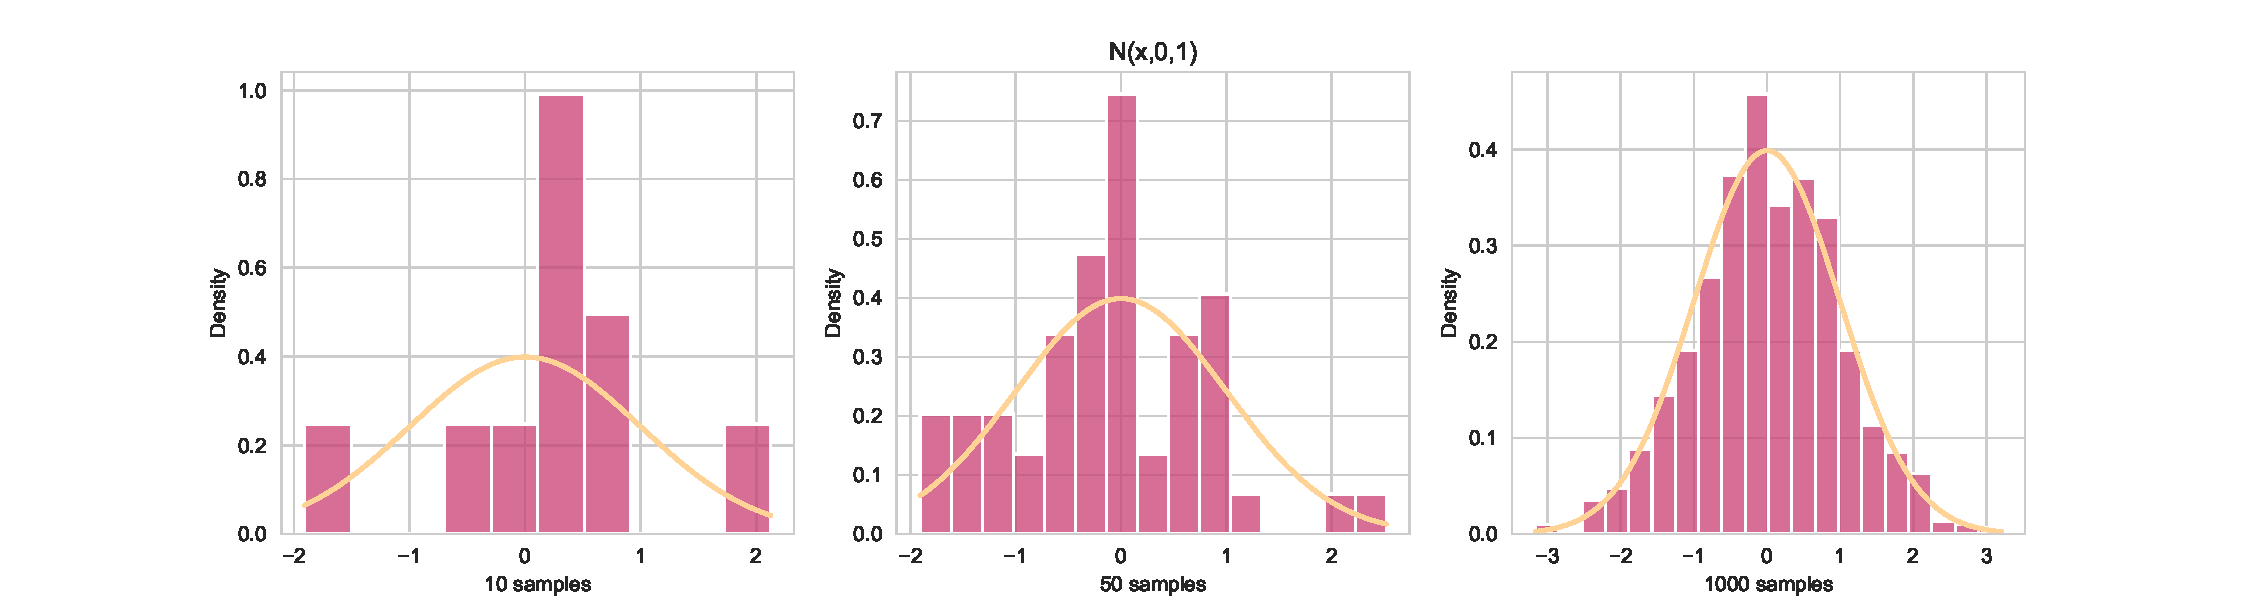
\includegraphics[width = 18 cm]{images/normal.pdf}\caption{Нормальное распределение}\label{figure1}
\end{center}
\end{figure}

\begin{figure}[H]
\begin{center}
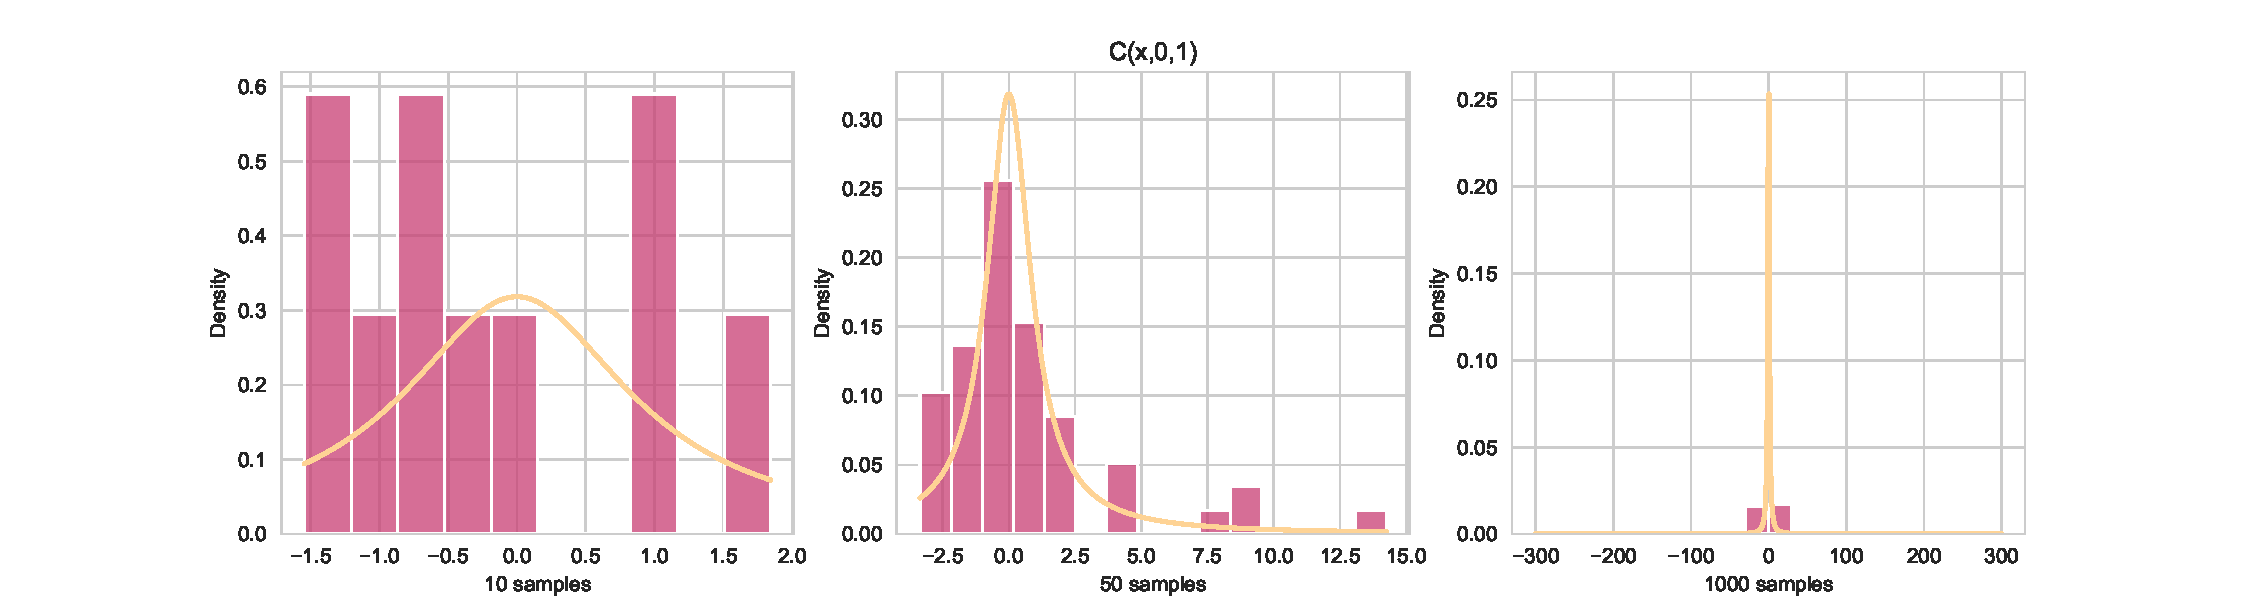
\includegraphics[width = 18 cm]{images/koshi.pdf}\caption{Распределение Коши}\label{figure1}
\end{center}
\end{figure}

\begin{figure}[H]
\begin{center}
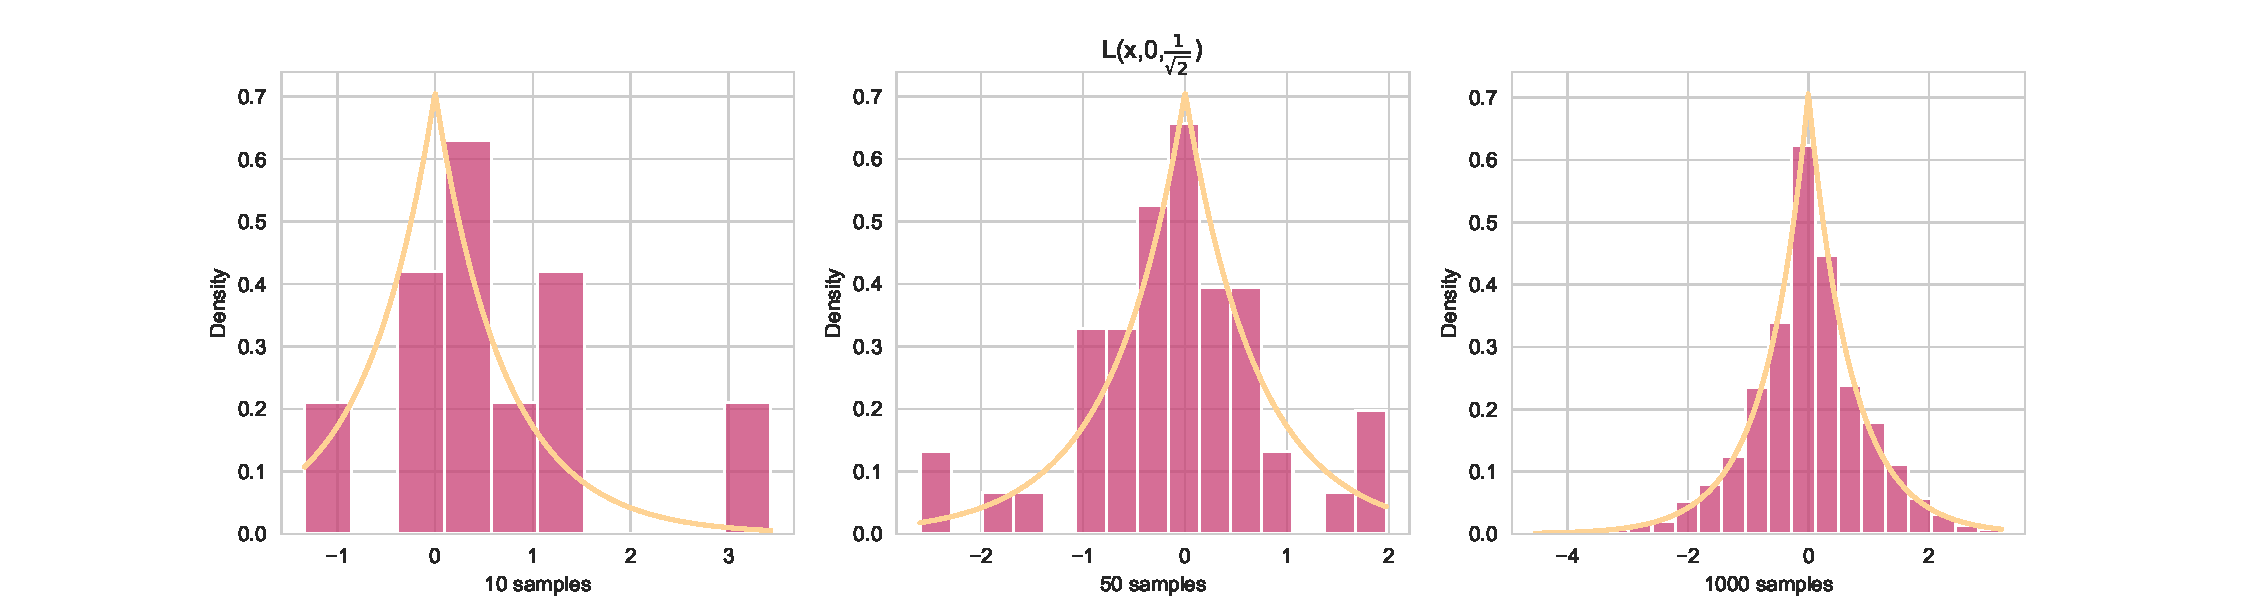
\includegraphics[width = 18 cm]{images/laplace.pdf}\caption{Распределение Лапласа}\label{figure1}
\end{center}
\end{figure}

\begin{figure}[H]
\begin{center}
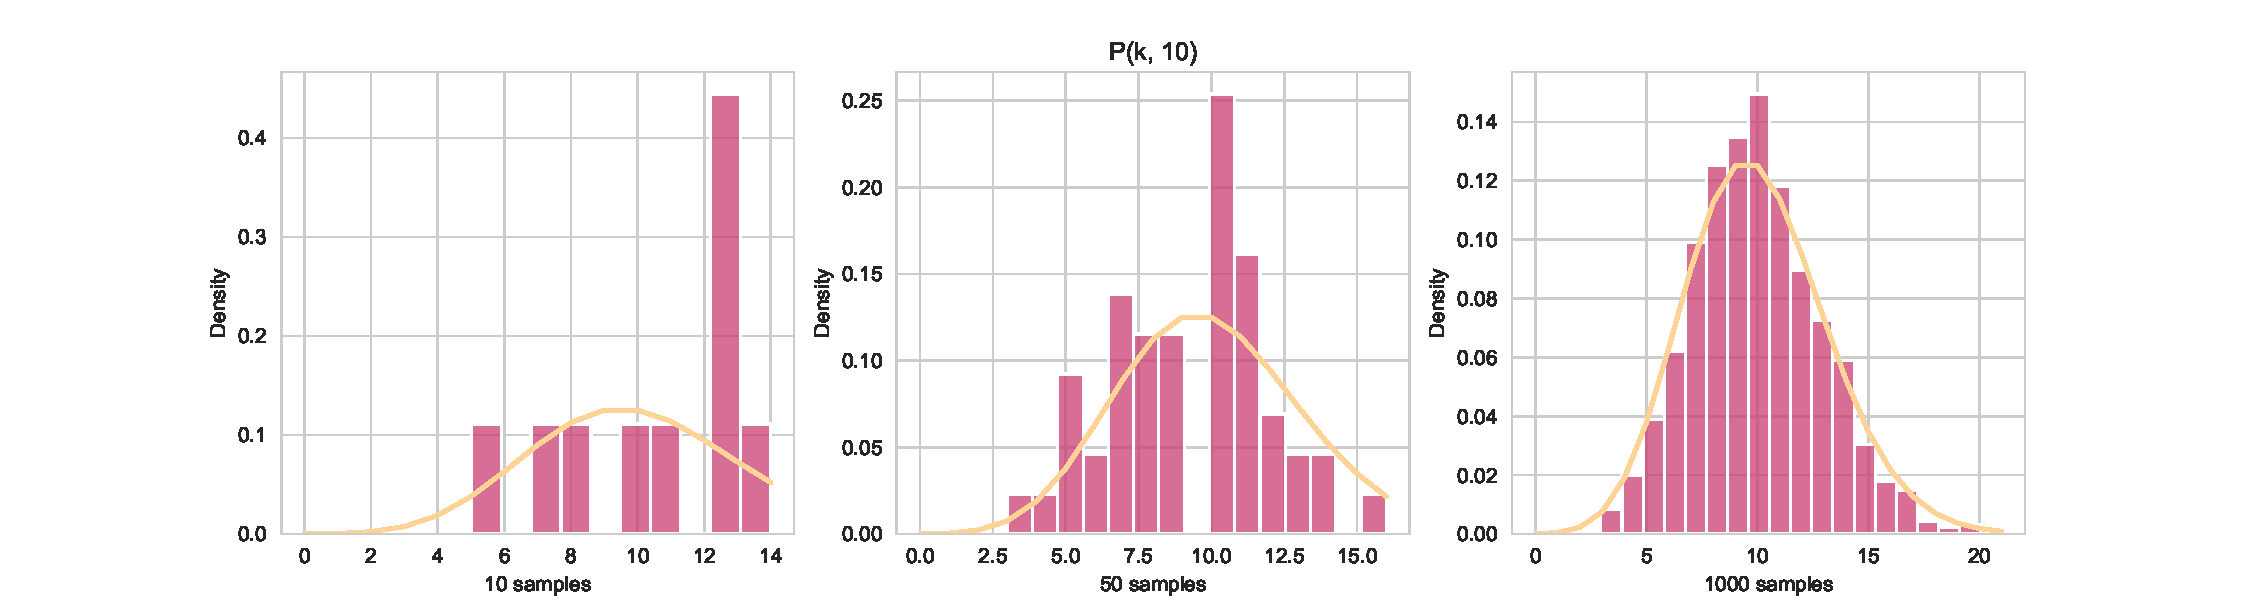
\includegraphics[width = 18 cm]{images/poisson.pdf}\caption{Распределение Пуассона}\label{figure1}
\end{center}
\end{figure}

\begin{figure}[H]
\begin{center}
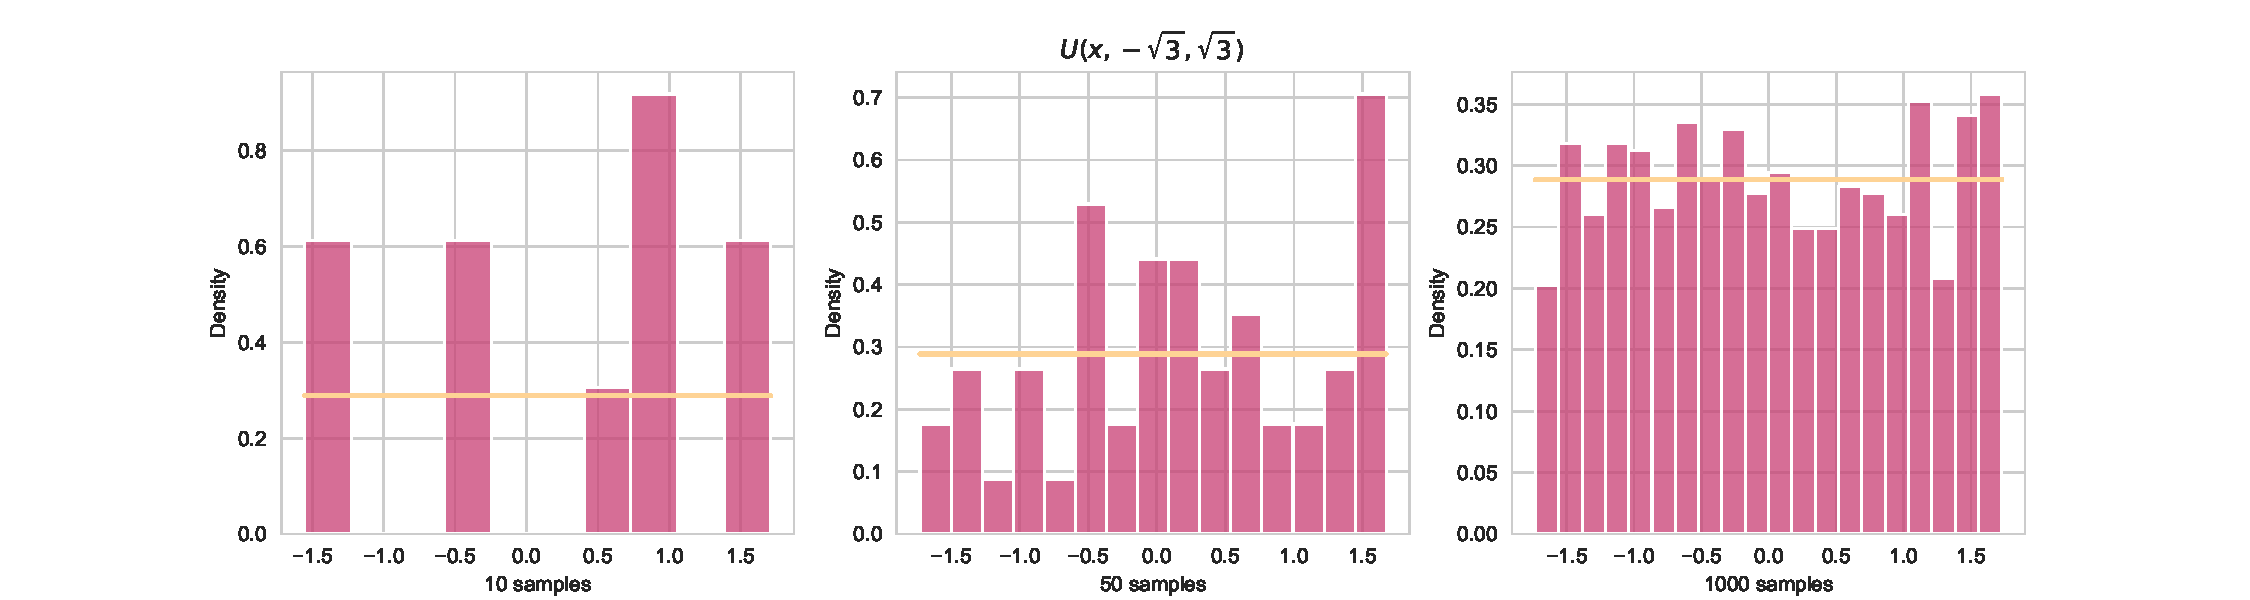
\includegraphics[width = 18 cm]{images/uniform.pdf}\caption{Равномерное распределение}\label{figure1}
\end{center}
\end{figure}

\section{Обсуждение}
Из результатов проделанной работы можно сделать вывод о том, что маленькая выборка не репрезентативна и по ней нельзя определить характер распределения исследуемой величины. При этом чем больше выборка - тем ближе гистограмма к плотности распределения и тем реже встречаются всплески.

\section{Приложение}
 Код программы GitHub URL:\\
 https://github.com/Elizaveta11111/MathStatistic/blob/main/Lab1/main.py

\end{document}
